
\qquad
\pagestyle{empty}
\newpage

%
%\chapter*{Introduction}
%
%%\begin{flushright}
%%\emph{Within a few years a simple and inexpensive device, readily carried about, will enable one to receive on land or sea the principal news, to hear a speech, a lecture, a song or play of a musical instrument, conveyed from any other region of the globe.}\\ -Nikola Tesla, 1905. 
%%\end{flushright}
%%\vspace*{0.6cm}
%
%Since early anatomical studies, reproduction of images has been one of the main tool to investigate structures and differences in organs and organisms. 
%Better ways to represent reality have undoubtedly led to better ways to understand it, and the pioneers' work in each discipline sharing the common need for precise and detailed images, were aided by available techniques offered in every epoch. 
%\begin{figure}[!ht]
%	\centering
%	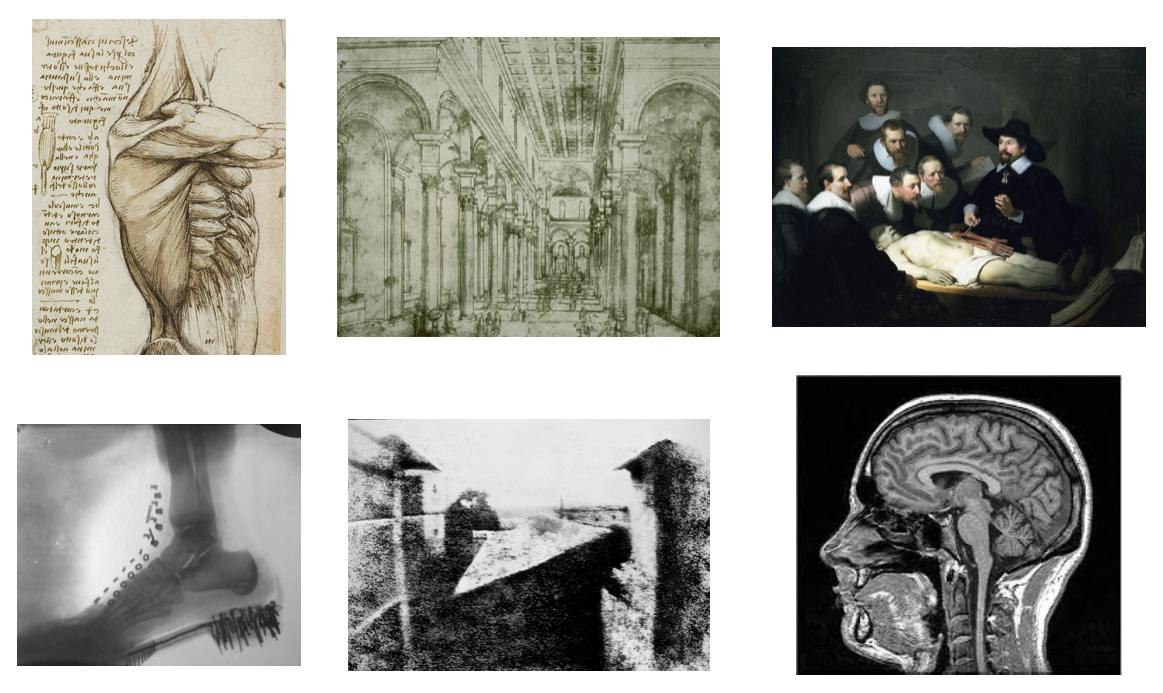
\includegraphics[scale=0.35]{figures/image_evolution.png}
%	\label{fig:evolution}
%\end{figure}  
%
%\noindent
%At the dawn, not surprisingly Artists and Anatomists could have not be separated, and every enhancement made in one field followed immediately others in other disciplines.
%Although semantics to differentiate fields of knowledge and art varied according to the epoch, the origin of every improvement in images ability reproduction has its roots in the study of Geometry.\\
%The first and most significant example is the powerful idea of perspective. Fixing a point from where to start infinitely parallel straight lines, leads, 16 centuries after their formalizations, Brunelleschi to revolutionize the  world's perception in artists' minds.
%Two centuries later, when the inventors' work took the name of Science, the study of magnifying lenses and their combination, made available new explorable territories. Here again the Geometry couldn't have more important role in the systematic study of the lights deformation effect through conic-shaped glass, and in the study of light itself  by Newton and Hyugens.\\
%Growing number of needs grows skills and techniques: artist, scientist and anatomist could not stay anymore below the same person's name, but what has remained constant is that every new discovery and improvement in one field became an immediate advancement in others.
%With the first stages of photographic techniques in the early '800, in parallel with the Young double slit experiment and its Fresnel interpretation, scientific community enhanced his attention to the shape of light. In late years of the same century the elegant Maxwell unification and its formalization by Heaviside determined the geometrical parameters of light. The discovery of X-ray by the first Nobel prize Roentgen and its refinement by Tesla is considered \cite{bradley2008history} the birth certificate of Medical Imaging, a domain destined to walk hand by hand with physics and engineering and to be eventually the most collaborative and crossing discipline ever seen. The transition from pencil's scientists and painting's artists to photographic equipment that characterizes this period did not impact only this newborn branch. Instruments brings literally light on the severe limits of human eye capabilities: what was hidden reality become visible. \\
%Just after the formalization of electric and magnetic field's shape, and the consequent mastery of electrical forces, the discovery of photoelectric effect opened new fields in the Physics of matter and a consequent new reformulation of mechanics far beyond the Cartesian space's Geometry, both in bigger and smaller scale. With the new interpretation of diffusion processes, there was been defined all the angular theories used also in the construction of fundamental equipment for medical imaging.\\
%In the wake of the third industrial revolution, electronic engineering, with its radio circuits, triods and valves destined to became transistor, provided each time better instrument to medical science where the acquisition and manipulation of patient images is a thriving theme. 
%Thanks to philanthropic, scientific and economic interest gravitating around health care, the complicated interaction between sciences, physics and medicine get smoothed leading to achievement as radiography, ultrasound, thermography, magnetic resonance, optical fiber, nuclear medicine, confocal microscopy just to name a few. Technologies aimed to visualize the interior of a body always attained from several parts to reach their aims. \\
%When photography get rid of photosensitive films to welcome digital sensors, images become stored in byte's grids with consequent powerful manipulation possibilities. The translation of acquired data from several sources, not always or entirely compatible with the human sight, to a suitable form meets new challenges.
%This is the context in which Machine Vision and Image Processing make their entrance; among the various advanced techniques, they provide two tools mostly utilized in medicine to reveal internal features and compare anatomies. Segmentation and registration suit as natural instrument in the investigation of patients' anatomies and physiologies. \\%Segmentation consists in enhance contours, detect edges and reveal hidden structure. .\\
%This Master Thesis deals with diffeomorphic image registration and, letting aside dribs and drabs history of science, still a few words about the state of the art are needed to complete its introduction.

\section*{An ill-Posed Problem}


Two instruments from Machine Vision and Image Processing are mostly utilized in Medical Imaging to reveal internal features and compare anatomies: segmentation and registration. Segmentation consists in enhance contours, detect edges and reveal hidden structure while registration is the process of determining correspondences between two or more images acquired from patients scans.\\
Dealing with image registration problem means search for a solution to an ill-posed prob- lem. Transformations between anatomies are not unique, and the impossibility of recover the spatial or temporal evolution of a anatomical transformation from temporally isolated images, makes any validation a difficult, if not impossible task. Among all of the possible voxelwise mappings that transform one image into another, interest may vary according to the requirements of each specific clinical situation\footnote{A recent survey in medical image registration can be found in \cite{Sotiras:survey:13}.}.\\
%
%%\section*{Toward an Ill Posed Problem Solution}
%Two instruments from compute vision and image processing are mostly utilized in Medical Imaging to reveal internal features and compare anatomies: image segmentation and image registration. %appears as the most natural tools in the investigation of patients' anatomies and physiologies. \\
%Segmentation consists in enhancing contours, detecting edges and revealing hidden structure, while registration is the process of determining spatial transformations between two or more images acquired from patients scans. Examples of such transformations are  Each spatial transformation is identified by specific set of parameters whose dimensionality depends on the complexity of the registration problem.\\
%Among all of the possible voxelwise transformations that maps one image into another, interest may vary according to the requirements of each specific clinical situation\footnote{A recent survey in medical image registration can be found in \cite{Sotiras:survey:13}.}. \\
%
%% Intra patient and inter patient.
%
%In both cases, dealing with image registration problem means searching for a solution to an ill-posed problem. Indeed, transformations between anatomies are not unique, and the impossibility of recovering the spatial or temporal evolution of an anatomical transformation from a succession of images, makes any validation a difficult, if not impossible task. 
%
%
In brain imaging, for example, registration can be performed to examine differences between subjects and distinguish affected from unaffected patients. This often results in a better understanding of the disease's features. Another case may require to compare different acquisition of the same subject, before and after a surgery or after a fixed period of time: in each case parameters and features of the transformation are completely different.
Customized registration techniques are required also when dealing with distortion motion correction caused by cardiac pulses or respiratory cycles, or for the mosaicing of several images acquired with a limited field of view, for example through a optical fiber probe.
Also the correction of motion distortion in image's acquisition phase, the mosaicing of several images or the construction of the model of cardiac and respiratory motion require customized image registration techniques.\\
Any approach is therefore varied and flexible: this led to a wide range of variants that has been proposed by researchers in the last decades\footnote{A quick glance to Google scholar reveals about $1200000$ papers in \emph{medical image registration} (55\% of the whole \emph{image registration} resources).}.\\
There are several features that distinguish image registration's algorithms, but the most relevant it is the choice of the family to whom the transformation belongs. Since anatomies are in a continuous process of modification over time, in general without any variation in the topological features, the use of diffeomorphisms to model transformation appears one of the most natural.\\
Continuous nature of these functions appears to be in contrast with the discrete nature of voxel images as well as with any computer's parametrization ability.\\
The approach of modeling with richer structure for simpler elements is actually very common even in everyday math: for example when measuring the diagonal of a $1$ meters side squared table. The decimal unlimited non periodical $\sqrt{2}$ doesn't help until we don't consider it as an answer belonging to a larger-than-reality mathematical structure: computations and theorem (as the Pythagorean one) are well defined and meaningful.\\ 
The simple structure of a raster image as 3-dimensional matrix is really limited if compared to the continuous object they represent. Modeling with continuous function provides a structure that reflects the object's reality. In addition enable us to apply mathematical features from differential geometry and dynamical system theory.\\
The first idea of using smooth and continuous function for image registration goes back to the idea of using the Navier-Cauchy partial differential equation to model the deformation of images as two balancing forces applied to an elastic body \cite{Broit:1981}. The solution's domain restriction to diffeomorphisms for the solution of the Lagrange transport equation for medical imaging registration appears in \cite{Dupuis:98:variationalproblems} and \cite{Trouve:98}, and with his many variants is an active subject of study for research in mathematic applied to medical imaging.
An important framework for the computation of image registration of diffeomorphism is provided by the Large Deformation Diffeomorphic Metric Mapping (LDDMM). Here diffeomorphisms are parametrized as ending point of integral curves of vector field on the Lie group of diffeomoprhism equipped with a Riemannian metric \cite{dupuis1998variational}, \cite{beg2005computing}. In this framework, solid mathematical foundations are payed in term of computational complexity. Aimed to solve this issue, different parametrization of diffeomorphisms, as Stationary Velocity Fields \cite{arsigny2006statistics} has been embedded in the LDDMM framework. This approach gave birth to the DARTEL \cite{Ashburner:07} and the Stationary LDDMM \cite{hernandez2007registration}. Starting from the Tririon's DEMON algorithm \cite{thirion1998image}, a different framework for diffeomorphic image registration was presented as Diffeomorphic Daemon \cite{vercauteren2007non} and the LCC-daemon \cite{lorenzi2013lcc} . A comparison between stationary LDDMM and Diffeomorphic Demons with emphasis in both theoretical and practical aspects can be found in \cite{hernandez2008comparing}. \\
The theme of diffeomorphism do not recurs only in medical application but it is a continuously improved subject of research also theoretical studies as \cite{Milnor:84:remarks}, \cite{bauer2011geodesic}, \cite{bauer2010sobolev} or studies applied to other domains of science \cite{Arnold:Khesin:14} \cite{ovsienko1992integrals}. Geometry remains an important underpinning structure for many achievement in medical imaging and advanced researches are actively utilized for applications.\\
from the necessity of having statistics to infer the variability of anatomical structure while performing image registration, bring the field of Patter Analysis from Machine Vision to Medical Imaging, with the name of Computational Anatomy (cite survey computational anatomy). 
Statistics on diffeomorphisms are introduced using a metric space defined over the Lie algebras of the Lie group of diffeomorphisms: this idea took the name of log-euclidean framework. Proposed for the first time in 2004 and refined in by the same authors in 2006 \cite{Arsigny:MRM:06}, as a faster improvement to the affine invariant Riemannian approach, has found successful applications in many domains of medical imaging (in vivo mosaicing \cite{Vercauteren:PHD:08}, brain Alzheimer detection \cite{Lorenzi:PhD:12}, cardiac image analysis \cite{Mansi:IJCV:11}, mandible imaging using polyaffine registration \cite{Seiler:MICCAI:11}) and has been continuously improved.\\
Thus the use of diffeomorphisms brings several aspect to be studied and to consider in their utilization:
theoretical research, their practical utilization, their study in statistical analysis and in the anatomical deformations' evolutions.\\
In this thesis we investigate some numerical methods to compute their composition in the log-euclidean framework aimed to the diffeomorphic image registration. Numerical computations are performed using parallel transport and accelerating convergence series, and are compared with the currently used BCH formula, keeping into account theoretical and practical aspects of the matter.

% % % % % % % % % % % % % % % % % % % % % % % % % % % % % % % % % % % % % %
% % SUB SECTION
% % % % % % % % % % % % % % % % % % % % % % % % % % % % % % % % % % % % % %
\section*{Thesis' Organization and No(ta)tions}

The first chapter about the general framework in image registration and parametrization of diffeomorphisms for LDDMM and SVF is followed by three distinct part. The first one presents basic tools of differential geometry and parallel transport, with emphasis on the computational side. The second part is about the principal objects utilized to explore new numerical techniques and to compare them with the one currently utilized. The last part is devoted to the results for the computation on synthetic dataset and on patient images. \\

\begin{enumerate}
	\item[{\bf Chapter \ref{se:registration_framework}:}] Introduction of the registration framework. After a first section about the main definitions and concepts utilized throughout the thesis, general registration framework's features are presented. Particular attention is given to the pros ad cons of in the use of diffeomorphism as set of transformation between anatomies and some considerations about methods currently used for their parametrization: the LDDMM and SVF. 
	
	\item[{\bf Chapter \ref{ch:finite_lie_group}:}] Possibilities of transformations' set when provided by mathematical structure of Lie group. Main mathematical elements and tools from Lie group theory directly involved in the image registration techniques are formally defined with a particular attention to flows, left translation, push forward, Lie logarithm and Lie exponential. We define the concept of Log-composition around which the research gravitates: it originates form the need of generalized the BCH formula. In this context the BCH become one possible way to compute the Log-composition. The second way to compute it in finite dimensional case, is provided by the Taylor expansion, presented in the last section.
	
	\item[{\bf Chapter \ref{ch:parallel_transport}:}] BCH and Taylor expansion are two possibility to compute the Log-composition. A third one presented in this chapter originates by a geometrical approach and it is given by the parallel transport. First and Second sections are devoted to present the theoretical tools to define formally the parallel transport. Last section is about two strategies to compute the parallel transport without involving the Christoffel symbols: the Schild's Ladder and the Pole Ladder.
	
	\item[{\bf Chapter \ref{ch:accelerating}:}] xxx
	
	\item[{\bf Chapter \ref{ch:rigid_body_transformations} and \ref{ch:svf}:}] Validity of results in the Log-composition computations are tested with two groups of transformations commonly used in medical image registration: the group of rigid body transformation and the group of diffeomorphisms (expressed in the application as the set of Stationary Velocity Fields). These chapters are aimed to present them in details and they are oriented to the application. 
	
	
    \item[{\bf Chapter \ref{ch:application_log_composition}:}] This is the central part of the research. The Log-composition is analyzed as s valuable tool in image registration, within the framework presented in chapter \ref{se:registration_framework}. A summary of the methods for its computation is presented as possible numerical approximation to be utilized for image registration: BCH formula, Taylor expansion, parallel transport and Accelerating Convergences series. 
    
     \item[{\bf Chapter \ref{ch:lie_log_computation}:}] The algorithm for the Lie-logarithm computation presented in \emph{A new algorithm for the computation of the group logarithm of diffeomorphism} \cite{Bossa:08} is based on the computation of the BCH formula. If reformulated with the Log-composition, each of its numerical approximation is a valid tool to improve its performance. Of particular interests are the methods that avoid the computation of the BCH formula on which the algorithm was initially based.
     
	\item[{\bf Chapter \ref{ch:results}:}] This chapter is devoted to experimental results. Performance of the Log-composition applied to rigid body transformation and diffeomorphisms are separately computed and compared. In addition a version of NiftyReg based on various we present the results of the numerical methods presented in the previous section, on synthetic data as well as on clinical data within a version of the  LCC-Demons customized with parallel transport.
	
	\item[{\bf Chapter \ref{ch:conclusions}}] Conclusion of what has been done so far (with a shameless and challenging emphasis of what is missing and what is still to be done).

	
	
\end{enumerate}








